\begin{minipage}[b]{0.8\textwidth}
\begin{Exercise}[title = Zwei Pucks, origin = {Morin - Classical Mechanics}, difficulty = 3, label = pucks]
Ein masseloser Faden der Länge $2\ell$ verbindet zwei Hockeypucks, die auf einer reibungsfreien Eisfläche liegen.\\
Jemand zieht mit einer konstanten Kraft $\vec{F}$ an der Mitte des Seils, wobei die Kraft senkrecht angreift.
Nach einer gewissen Zeit stoßen die beiden Pucks komplett inelastisch zusammen. Wie viel Energie geht bei dem Stoß verloren?
\end{Exercise}
\end{minipage}
\hfill
\begin{minipage}[b]{.2\textwidth}
\centering
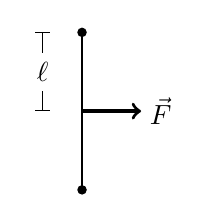
\begin{tikzpicture}
\filldraw (0,1) circle (1.5pt);
\draw (0,1) -- (0,-1);
\filldraw (0,-1) circle (1.5pt);
\draw[->,very thick] (0,0) --  (0.75,0);
\node at (1,0) {$\vec{F}$};
\draw[|-|] (-.5,1) to node[midway, fill = white] {$\ell$} (-.5,0);
\end{tikzpicture}
\end{minipage}
